\chapter{Stage}
\textit{Questo capitolo spiega il motivo per cui l'azienda ha deciso di pendere uno stagista e l'utilità che potrà avere nella realizzazione del progetto. Inoltre, vengono presentati i vincoli imposti in sede di pianificazione dello stage e gli obiettivi che ci si aspetta vengano realizzati.}

\section{Vantaggi dell'azienda}
Tepui trae diversi vantaggi dall'attività di stage curricolare organizzata presso la sede di Castelfranco Veneto.

In primo luogo, l'aumento della forza lavoro. L'introduzione di un nuovo membro nel team di sviluppo ha permesso all'azienda di redistribuire il carico di lavoro in modo da implementare altri progetti in cantiere e di incrementare i servizi di consulenza. Inoltre, il punto di vista proveniente da un utente esterno ha permesso all'azienda di individuare nuove funzionalità di Instant Developer rilasciate dalla casa produttrice.
Un esempio di nuova funzionalità è stata la realizzazione del caricamento immagini senza l'ausilio di informazioni di header in fase di upload e la possibilità di caricare i file in una cartella specifica temporanea modificando dei comandi preimpostati dall'applicazione.

In secondo luogo, lo stage ha permesso all'azienda di apprendere un metodo di implementazione del codice ordinato attraverso la catalogazione offerta da InDe che dà la possibilità di includere parti codice in cartelle e sottocartelle scrivendo a commento la loro funzionalità in modo che il codice sia più facile da capire.

In terzo luogo, il costo di uno stagista è stato minimale ed ha permesso di esplorare nuove funzionalità risparmiando. Trattandosi di un'azienda giovane, poter conoscere e migliorare la propria operatività a prezzi irrisori è considerato un'ottima occasione. 


\section{Presentazione del progetto}
In questa sezione verranno esposte le informazioni di base relative al progetto da realizzare. Entreremo nel dettaglio del progetto nel capitolo 3.
\\

Il progetto da realizzare rappresenta una applicazione web che permetta ad una azienda cliente di inserire e mantenere un catalogo prodotti lato back-end, ovvero inserire informazioni che verranno utilizzate dalla pagina web alla quale accedono i consumatori B2B. 
Il progetto in questione quindi mira a:
\begin{itemize}
	\item semplificare l'inserimento a database dei dati che verranno utilizzati da un'altra applicazione;
	\item arricchire dati provenienti da un sistema terzo.
\end{itemize}

Il progetto si compone di un insieme di schermate che devono offrire la possibilità di gestire tutti i prodotti di un catalogo. 


\begin{figure}[!h] 
	\centering 
	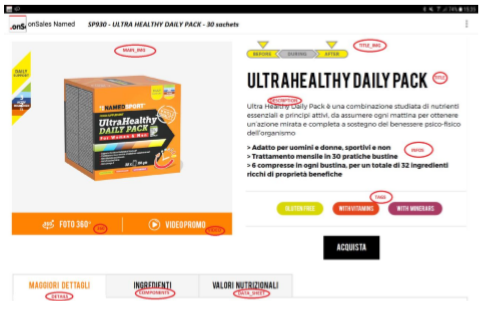
\includegraphics[width=1\columnwidth]{frontend} 
	\caption{Front-end realizzato con i dati inseriti dal configuratore}
	\label{ImgFrontend}
\end{figure}

\subsubsection{Visualizzazione prodotti}
Nella schermata di "Visualizzazione prodotti" si devono presentare i singoli articoli e alcune delle informazioni più importanti tra cui il codice identificativo, nome breve del prodotto e a quali famiglie di prodotti esso appartiene. In questa videata è richiesta la presenza delle seguenti operazioni: ricerca, cancellazione, inserimento e dettaglio.
Per quanto riguarda l'inserimento esso può avvenire direttamente nell'elenco prodotti indicando gruppo di appartenenza, codice e nome breve.
Entrando nel dettaglio invece, è richiesta l'apertura di una seconda schermata riempita con i contenuti del prodotto presenti nel database, quindi gestire le informazioni che si desiderano presentare nella pagina web di front-end.
Un'altra operazione a cui bisogna prestare attenzione è la cancellazione di un prodotto. Il cliente ha chiesto espressamente che questa cancellazione sia unicamente logica per quanto riguarda il prodotto fatta eccezione alle informazioni interne che potranno essere cancellate fisicamente: tag, specifiche tecniche del prodotto, immagini.

\subsection{Visualizzazione dettaglio prodotto}
La "Visualizzazione dettaglio prodotto" rappresenta il centro del progetto. In questa schermata devono essere implementate diverse funzionalità che permettono di gestire al meglio l'inserimento e l'aggiornamento delle informazioni di un articolo. Fondamentale è nella schermata avere un'unico metodo di salvataggio e dei controlli specifici che creino unicamente i record necessari. 
Le informazioni che bisogna essere in grado di gestire sono:
\begin{itemize}
	\item Nome esteso, descrizione ed informazioni;
	\item Inserimento e gestione tag;
	\item Inserimento e gestione immagine principale;
	\item Inserimento e gestione video;
	\item Inserimento e gestione Titolo (immagine);
	\item Inserimento e gestione immagine/i 360, ovvero la creazione di una galleria di immagini da mostrare;
	\item Informazioni aggiuntive che possono essere create, modificate e cancellate da una schermata a parte.
\end{itemize}

\subsection{Inserimento attraverso modali}
Gli inserimenti delle immagini, video o delle informazioni aggiuntive deve avvenire attraverso delle modali. Le modali richieste prevedono l'inserimento di queste informazioni: Numeri, Liste valori, Stringhe, Date, Booleani, Multi-selezione, URL, Email, Telefono, File, Immagine, Multi-File, Immagini 360.

\subsection{Gestione delle configurazioni}
Le informazioni che devono poter essere aggiunte ad un prodotto hanno dei record preimpostati non cancellabili. Inoltre con questa schermata nasce l'intento di poter creare tipi di informazioni aggiuntive a discrezione dell'utente finale.
Nell'inserimento dell'informazione da gestire è necessario limitare l'utente con i tipi indicati nelle modali.

\subsection{Gestione delle traduzioni}
Al termine del progetto è richiesto di individuare un metodo adeguato per la gestione delle traduzioni dei prodotti in lingue differenti dall'italiano. Studio dell'eventuale utilizzo di una componente RTC presente su InDe con una licenza da acquistare.

\subsection{Altri interventi}
Infine, oltre alla realizzazione del progetto, l'azienda per rendere lo stage vicino alla realtà che deve affrontare ogni giorno ha chiesto di essere disponibile e pronto a fornire supporto in questioni esterne al progetto che possono verificarsi.


\subsection{Obiettivi}
Gli obiettivi concordati nel piano di lavoro sono stati suddivisi in tre categorie: obbligatori, desiderabili e facoltativi. L'azienda ha espresso la richiesta che gli obbligatori siano completati, mentre per i desiderabili, almeno due dei tre indicati, siano portati a termine. \\
 
Gli obiettivi si distinguono in:
\begin{itemize}
	\item Obbligatori
	\begin{itemize}
		\item \underline{\textit{O01}}: Apprendimento della piattaforma Instant Developer;
		\item \underline{\textit{O02}}: Test delle funzionalità implementate e rilascio;
		\item \underline{\textit{O03}}: Utilizzo di Microsoft SQL Server.
	\end{itemize}
	
	\item Desiderabili 
	\begin{itemize}
		\item \underline{\textit{D01}}: Gestione di progetto;
		\item \underline{\textit{D02}}: Comunicazione con il cliente;
		\item \underline{\textit{D03}}: Scrittura delle procedure T-SQL.
	\end{itemize}
	
	\item Facoltativi
	\begin{itemize}
		\item \underline{\textit{F01}}: Autonomia a risolvere nuove problematiche.
	\end{itemize} 
\end{itemize}


\section{I vincoli}
\subsection{Vincoli temporali}
Lo stage ha una durata prevista di 310 ore complessive, distribuite in 8 settimane da 40 ore lavorative ciascuna, dal 13 Maggio 2019 al 8 Luglio 2019. L'orario di lavoro concordato con il tutor aziendale è stato dal Lunedì al Venerdì dalle 09:00 alle 18:00, con 1 ora di pausa pranzo. Prima dell'inizio dello stage è stato redatto un piano di lavoro con una scansione temporale delle attività con granularità settimanale così definita:


\begin{figure}[!h] 
	\centering 
	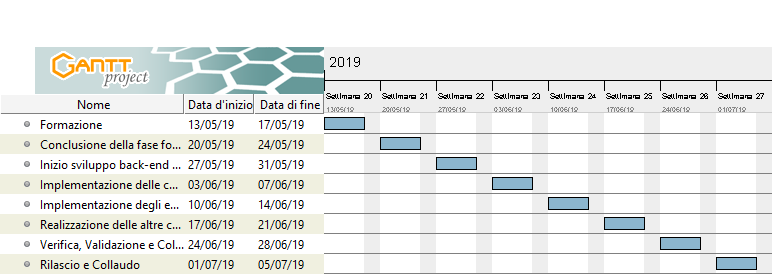
\includegraphics[width=1\columnwidth]{diagrammagantt} 
	\caption{Diagramma di Gantt}
	\label{Gantt}
\end{figure}


\subsubsection*{Prima Settimana - Formazione (40 ore)}
La prima settimana prevede l'apprendimento del programma Instant Developer seguendo un corso online composto da video realizzati dai produttori del programma. Inoltre, per apprendere al meglio il prodotto, è richiesto che nel seguire il video si svolgano i progetti commissionati dal corso stesso integrandoli con richieste dell'azienda per velocizzarne l'apprendimento. 
Durante la settimana sono entrato in contatto con gli altri membri del team di sviluppo e ho compreso le dinamiche aziendali.

\subsubsection*{Seconda Settimana - Conclusione della fase formativa ed inizio gestione di progetto (40 ore)}
Durante la seconda settimana è stato previsto uno studio di SQL Server e delle stored procedure presenti nei database dell'azienda in modo da comprendere alcuni degli standard e saperli poi applicare in caso di necessità. Inoltre si inizia con la lettura delle specifiche del progetto che si dovrà realizzare e a seguito di una attenta analisi interna ci saranno degli incontri con il cliente per approfondire alcune caratteristiche su cui si desidera maggiore chiarezza. \\
Infine al termine della settimana ci si aspetta la redazione di un documento che riporti il metodo formativo dell'azienda se è stato sufficiente e dove si ritiene necessario maggior impegno in modo che tali documenti fungano da base per un loro miglioramento.

\subsubsection*{Terza Settimana - Inizio sviluppo back-end della componente (40 ore)}
La terza settimana si entra nella progettazione che prevede una prima comprensione del problema e realizzazione di una bozza delle tabelle da creare al fine di non compromettere il sistema preesistente e integrando quello nuovo. Una volta individuate le tabelle necessarie dovranno essere implementate e in questa settimana si inizieranno a realizzare i primi documenti relativi a tempistiche e un primo aspetto grafico completo che il progetto dovrà avere.

\subsubsection*{Quarta Settimana - Implementazione delle componenti di base del progetto  (40 ore)}
Nella quarta settimana è stata prevista l'implementazione delle classi basate sulle tabelle ideate, le schermate ad esse associate e un giorno di riepilogo presso la sede del cliente dello stato di avanzamento del lavoro. Inoltre, internamente, hanno chiesto che si rediga un documento con le scelte implementative adottate per riutilizzare tale documentazione in caso di realizzazione di progetti simili o per sapere quali sono state le motivazioni che hanno portato ad una scelta implementativa rispetto ad un'altra.

\subsubsection*{Quinta Settimana - Implementazione degli eventi del progetto (40 ore)}
Nella quinta settimana è stato previsto un lavoro intenso nell'implementazione degli eventi di caricamento e salvataggio dei dati, mantenendo una costante redazione ed aggiornamento dei documenti relativi al progetto.

\subsubsection*{Sesta Settimana - Realizzazione delle altre componenti del progetto (40 ore)}
Durante la sesta settimana ci si aspetta che il prodotto sia sufficientemente sviluppato almeno per le componenti principali e quindi si dovranno effettuare i primi test di unità. Se il progetto è sufficientemente stabile inoltre sarà possibile passare alla creazione degli altri oggetti e delle altre schermate da realizzare, in particolare le schermate di upload delle immagini e dei file.
Nella settimana è previsto un incontro presso la sede del cliente in modo da visionare lo stato di avanzamento del prodotto commissionato.

\subsubsection*{Settima Settimana - Verifica, Validazione e Collaudo (40 ore)}
La settima settimana si presuppone che il progetto sia completamente realizzato e quindi si ricontrollino i documenti interni in modo che siano precisi al dettaglio per ogni singola schermata, classe e metodo implementato.
Poi si prevede l'integrazione del prodotto nel sistema preesistente con relativo collaudo di ogni singola funzionalità e quindi sistemazione degli eventuali bug del software.


\subsubsection*{Ottava Settimana - Rilascio e Collaudo (30 ore)}
L'ultima settimana si dedica al collaudo del software, alla pubblicazione di quest'ultimo al cliente perché possa testarlo e fornire eventuali feedback. Infine, sono previste in questa settimana la gestione di richieste particolari del cliente, come: miglioramento grafico ed eliminazione di funzionalità prima ritenute importanti.


\subsection{Vincoli metodologici}
In accordo con il tutor aziendale, lo stage si è svolto presso la sede dell'azienda. Questa decisione si deve principalmente a due motivi: 
\begin{itemize}
	\item Agevolare la comprensione, da parte dello stagista, delle dinamiche aziendali e l’interazione con il proponente del progetto; 
	\item Favorire il confronto tra stagista, team e tutor aziendale.
\end{itemize}
A seguito dei servizi di consulenza offerti dall'azienda, nella seconda metà dello stage, la comunicazione con il tutor è stata meno constante ed in previsione di ciò si è adottata la politica di individuazione ad inizio settimana dei task da sviluppare e ad ogni problema o implementazione completata una comunicazione nel canale Teams predisposto.

Per l'intera durata dello stage, \azienda\ ha richiesto che lo stagista redigesse delle brevi relazioni, descrivendo le problematiche affrontate, le scelte adoperate e il risultato ottenuto. Questi documenti hanno la funzione di materiale ausiliario dedicato al miglioramento della gestione degli stagisti.

Infine, é stato posto come obbligo che tutta la documentazione rimanesse in una cartella OneDrive e che ogni singola operazione svolta venisse indicata su iDo, la piattaforma con la quale riescono ad indicare le ore a consuntivo svolte per la realizzazione di ogni modulo.


\subsection{Vincoli tecnologici}\label{vincoliteconlogici}
Nella realizzazione del progetto l'azienda ha chiesto che si adottassero i concetti base della programmazione ad oggetti. In Instant Developer questo prevede che per ogni tabella del database debba essere creata una classe. Quindi si implementano solo ed unicamente metodi, che nel programma si distinguono in eventi e procedure, necessari. \\

\inde presenta due diverse modalità di creazione delle pagine web: Table Oriented (TO)\label{TO} e Document Oriented (DO) \label{DO}. Nel mio caso la richiesta dell'azienda prevedeva l'utilizzo della seconda modalità applicando i concetti appresi nella programmazione ad oggetti. La programmazione DO corrisponde alla Object Oriented Programming (OOP)\label{OOP}.

La DO si basa su un framework ORM (Object-relational Mapping) di classe enterprise, il cui scopo è, oltre quello di automatizzare il caricamento degli oggetti dal database, quello di gestirne l'intero ciclo di vita e le relazioni con gli altri componenti dell'applicazione. Le caratteristiche enterprise della DO sono arricchite dalla presenza di un sistema estensibile di servizi ai documenti, che attraverso tecniche OOP permette di implementare caratteristiche comuni alla gerarchia delle classi \hyperref[bib11]{\cite{[11]}}.

Con InDe è possibile creare manualmente le classi e poi aggiungere le proprietà e i metodi, oppure affidarsi ad un metodo più semplice, ovvero quello di effettuare un D\&D della tabella del database che conterrà i dati del documento sull'applicazione, tenendo premuti i tasti shift e ctrl, generando automaticamente le classi. 

Questo comportamento dell'applicazione va contro i principi dell'ingegneria del software, la quale prima prevede si progetti lo schema delle classi e poi questo lo si traduca in uno schema di database. Il metodo proposto non presuppone una maggiore importanza del database rispetto alle classi, ma è stato pensato per ottenere i seguenti vantaggi \hyperref[bib11]{\cite{[11]}}:
\begin{itemize}
	\item il database è già presente; con l'importazione ottengo lo schema del database e genero classi in maniera automatica;
	\item se il database è nuovo, la sua definizione dovrebbe seguire gli stessi principi della	creazione dello schema delle classi; quindi partire da un punto o dall'altro è indifferente;
	\item dal punto di vista del framework DO, esso utilizza anche alcune informazioni presenti all'interno della definizione del database, come ad esempio la struttura delle
	foreign key.
\end{itemize}


\section{Scelta e obiettivi personali}\label{scelta e obiettivi}
Sono entrato in contatto con l'azienda ospitante grazie ad un amico che mi ha messo in contatto con i responsabili. Dopo un colloquio ed una spiegazione generale delle attività svolte dall'azienda, hanno suscitato il mio interesse. L'idea di interfacciarmi con il mondo del lavoro prendendo in mano la gestione di dati sensibili e la possibilità di creare un gestionale rientra perfettamente nell'impiego da me cercato.\\
Dopo aver studiato economia presso l'Istituto Tecnico Commerciale Statale P.F. Calvi ed informatica presso l'Università di Padova, entrare in una realtà lavorativa che concilia i due ambiti, mi sembra un buon completamento dei miei studi fino a questo momento.\\
Gli obiettivi che mi sono posto di raggiungere a livello personale oltre a quelli concordati con l'azienda sono: 
\begin{itemize}
	\item Accrescere le conoscenze in merito al mondo RAD e Data Warehouse;
	\item Migliorare le capacità di realizzazione di applicazioni seguendo il metodo Bottom-Up;
	\item Apprendere come interfacciarmi con i clienti;
	\item Migliorare le mie capacità di Problem Solving.
\end{itemize}

\newpage
